% Contributers: Carolina Zheng
\subsection{Hardness of k-means when k=2}
In class, we saw a proof that $k$-means is NP-hard for general $d$ and $k=\Theta(n)$. Now we will prove that $k$-means remains hard even when $k=2$. There is a simple proof in \cite{deshpande} that is a reduction from densest cut, which we will walk through in Theorem \ref{thm2}. Densest cut is equivalent to sparsest cut on the complement graph, which is known to be NP-complete \cite{matula1990sparsest}.

\begin{definition}[Densest cut]
    For a given graph $G=(V,E)$, find a bipartition $(P,Q)$ of the vertices in $G$ that maximizes $\abs{E(P,Q)}/(\abs{P}\abs{Q})$, where $E(P,Q)$ denotes the edge set of the cut.
\end{definition}

\begin{theorem}\label{thm2}
    $k$-means clustering in general dimension is NP-hard even for $k=2$.
\end{theorem}

Suppose we wish to compute the densest cut for a graph $G$ with no parallel edges. Define the $\abs{V}\times\abs{E}$ matrix $M$ as follows: entry $M[v,e]$ is zero if $e\in E$ is not incident on $v\in V$; otherwise, it is $+1$ for one endpoint $e$ and $-1$ for the other (it does not matter which endpoint is which).

Run $k$-means with $k=2$ on the set of points corresponding to the rows in $M$. Note that each point represents a vertex in $G$ and has dimension $\abs{E}$. Given an optimal solution to this $k$-means instance, we claim that two returned clusters correspond to the optimal bipartition $(P,Q)$ in densest cut. It is sufficient to show that minimizing the $k$-means cost on this instance is equivalent to maximizing the densest cut objective.

Let us compute the $k$-means cost for the two clusters $P$ and $Q$, where $|P|=p$, $|Q|=q$, and $p+q=n$. Denote points as $x\in \R^{|E|}$, where $x=(x_1,\dots,x_{|E|})$. Let $\mu^p$ be the centroid for $P$ and $\mu^q$ be the centroid for $Q$. Then $\mu^p=\frac{1}{p}\sum_{v\in P}M[v,:]$.

Consider $\mu^p_e$. If $e\not\in E(P,Q)$, then $\mu^p_e=0$, since if $e\in E(P,P)$, the nonzero values at the two endpoints will be summed together and cancel, and if $e\in E(Q,Q)$, all values that are summed are zero. If $e\in E(P,Q)$, then $\mu^p_e$ is either $\frac{1}{p}$ or $-\frac{1}{p}$, since the vertex incident on $e$ in $P$ will contribute either $1$ or $-1$ to the sum, and the vertex incident on $e$ in $Q$ will not be summed. Computing $\mu^q$ is analogous. In short,

\begin{equation*}
    \mu_e^p=\begin{cases}\frac{1}{p}\text{ or }-\frac{1}{p},&e\in E(P,Q)\\
                         0,&\text{otherwise}
            \end{cases}
\end{equation*}

Now we compute the $k$-means cost. Let $c(v)=p$ if $v\in P$ and $q$ if $v\in Q$.
\begin{align}\label{eq1}
    \text{cost}(P,Q)=\sum_{v\in P}\|M[v,:]-\mu^p\|^2+\sum_{v\in Q}\|M[v,:]-\mu^q\|^2 &= \sum_{e=1}^{|E|}\sum_{v=1}^{|V|}(M[v,e]-\mu_e^{c(v)})^2
\end{align}

Suppose $e\not\in E(P,Q)$. Fix $v$. Then $\mu_e^{c(v)}=0$, and $M[v,e]$ is nonzero iff $v$ is incident on $e$; in that case it is either $1$ or $-1$. Therefore the total cost over all vertices from $e$ is 2.

Suppose $e\in E(P,Q)$. Fix $v$. Suppose $v$ is not incident on $e$. Then $M[v,e]=0$ and $\mu^{c(v)}_e=\frac{1}{c(v)}$, so the cost is $\frac{1}{c(v)^2}$. There are $p-1$ such $v\in P$ and $q-1$ such $v\in Q$, so the total cost of the vertices not adjacent to $e$ is $(p-1)\frac{1}{p^2}+(q-1)\frac{1}{q^2}$. Suppose $v$ is incident on $e$. There are two such $v$, one of which is in $P$ and one of which is in $Q$. If $M[v,e]=1$, then $\mu^{c(v)}_e=\frac{1}{c(v)}$, and if $M[v,e]=-1$, then $\mu^{c(v)}_e=-\frac{1}{c(v)}$. Therefore the total cost of the two vertices adjacent to $e$ is $(1-\frac{1}{p})^2+(1-\frac{1}{q})^2$.

Adding the costs of all the edges together, the RHS of Equation \eqref{eq1} is equal to
\begin{align}
    &= \sum_{e\in E(P,Q)}[(p-1)\frac{1}{p^2}+\left(1-\frac{1}{p}\right)^2+(q-1)\frac{1}{q^2}+\left(1-\frac{1}{q}\right)^2] + \sum_{e\not\in E(P,Q)}2 \\
    &= \left(2-\frac{1}{p}-\frac{1}{q}\right)\abs{E(P,Q)}+2\abs{E(P,P)}+2\abs{E(Q,Q)} \\
    &= 2|E| - \frac{n}{pq}\abs{E(P,Q)}
\end{align}

Recall that $P$ and $Q$ are the clusters found by the $k$-means objective and their elements correspond to vertices in $G$. Since $|E|$ and $n$ are constants, the $P$ and $Q$ that minimize the $k$-means cost also maximize the densest cut objective in $G$. Similarly, the partition that maximizes the densest cut objective, when taken to be the two clusters in $k$-means, will minimize the $k$-means cost.

This completes the reduction from densest cut to $k$-means with $k$=2.
\qed

\subsection{Hardness of k-means when d=2}

Now we will prove that $k$-means is NP-hard even when $d=2$ and $k=\Theta(n^\epsilon)$ for $\epsilon>0$, following the proof in \cite{vattani}.

\textbf{Setup}. We consider the $k$-means clustering problem with weighted points. This is without loss of generality, since a point $x$ with weight $w$ can be replaced by $w$ distinct points very close to $x$. The following is the decisional version of the weighted $k$-means clustering problem.

\begin{definition}[Decisional weighted $k$-means]
    Given a multiset $S\subseteq \R^d$, an integer $k$ and $L\in\R$, is there a subset $T\subset\R^d$ with $|T|=k$ such that $\sum_{x\in S}\min_{t\in T}\|x-t\|^2\le L$?
\end{definition}

Analogously to what was noted in class, we can restate the cost of a cluster $C$ in terms of the points belonging to $C$, without referring to $T$. Specifically, let $w(x)$ denote the weight of point $x$. Then

$$\text{cost}(C)=\frac{1}{\sum_{x\in C} w(x)}\sum_{\{x,y\}\in\binom{C}{2}}w(x)w(y)\|x-y\|^2$$

The reduction will be from Exact Cover by 3-Sets (X3C), which is known to be NP-complete \cite{garey1979computers}.

\begin{definition}[Exact cover by 3-sets]
    Given a finite set $U$ containing exactly $3n$ elements and a collection $\cC=\{S_1,\dots,S_l\}$ of subsets of $U$, each of which contains exactly 3 elements, are there $n$ sets in $\cC$ such that their union is $U$?
\end{definition}

\textbf{Overview}. The bulk of our work will go to proving the following theorem.

\begin{theorem}\label{thm1}
The $k$-means clustering problem is NP-hard for $d=2$ and $k=\Theta(n^\gamma)$ for some $0<\gamma<1$.
\end{theorem}

We first give a high level overview of the reduction from X3C, namely the construction of a suitable $k$-means instance.

Let $l$ and $n$ be fixed (determined by the X3C instance). We set $k$ to be $l(3n+2)+(l-1)3n$. Then we place some points into the plane to form a grid, $H_{l,n}$. We define $w =\text{poly}(l, n)$ where $w$ is large enough relative to $l,n$, and define the distances and weights in $H_{l,n}$ in terms of $w$. We then argue that there are ``nice'' ways to cluster these points, such that the cost incurred is small relative to other clusterings. The minimal cost is $L_1-l\alpha$, where $L_1$ and $\alpha$ are defined in terms of $l,n$.

Then we add some more points from a set $X$ to a slightly modified version of $H_{l,n}$ to create $G_{l,n}\cup X$. These new points are related to the elements in $S_i$ for $S_i\in\mathcal{C}$. We then argue that iff the X3C instance is satisfiable, these new points can be clustered so that the total cost increases by an amount $L_2+(l-n)\alpha$ ($L_2$ defined in terms of $l,n$). Therefore our cost limit in the decision problem will be $L_1+L_2-n\alpha$, and we then argue that this is a valid reduction from X3C to $k$-means.

We will explain the above in detail in the next section. Given this construction, the $k$-means instance $G_{l,n}$ will contain exactly $l(6n+3)+(l-1)9n$ points, for which $k=\Theta(n^\gamma)$ for some $0<\gamma<1$ (according to the value for $k$ mentioned above; also note that the second $n$ here refers to the number of points in the $k$-means instance, not the $n$ in the 3XC instance). There is a simple reduction to the more general $k=\Theta(n^\epsilon)$ for some $\epsilon>0$.

\begin{theorem}
    Suppose Theorem \ref{thm1} is true. Then the $k$-means clustering problem is also NP-hard for $k=\Theta(n^\epsilon)$ for any $\epsilon>0$.
\end{theorem}

Fix $\epsilon>0$, and take a hard instance with $n$ points and $k$ centers, with $k=\Theta(n^\gamma)$ as in Theorem \ref{thm1}. The $\gamma=\epsilon$ case is trivial.

Suppose $\gamma<\epsilon$. Add $n^\epsilon$ points very far from the original instance and very far from each other, and $n^\epsilon$ centers. The optimal solution will use the new centers to cluster the new points, and the optimum in the original instance will not change. Therefore this is a hard instance with $m = n+n^\epsilon=\Theta(n)$ points and $k'= k+n^\epsilon=\Theta(n^\epsilon)$ centers.

Suppose $\gamma>\epsilon$. Add $n^{\gamma/\epsilon}$ points very close to each other and far from the original instance, and 1 center. The optimal solution will use the new center to cluster the new points, and the optimum in the original instance will not change. Therefore this is a hard instance with $m= n+n^{\gamma/\epsilon}=\Theta(n^{\gamma/\epsilon})$ points and $k'= k+1=\Theta(n^\gamma)=\Theta(m^\epsilon)$ centers.\qed

\textbf{Proof of Theorem \ref{thm1}}. We construct the grid $H_{l,n}$, which is depicted in Figure \ref{fig:vattani1}. We create ``rows'' $R_i$ ($1\le i \le l$) alternated with rows $M_i$ ($1\le i \le l-1$). Each row $R_i$ is composed of $6n+3$ points $\{s_i,r_{i,1},r_{i,2},\dots,r_{i,6n+1},f_i\}$, where $s_i,f_i$ weigh $w^2$ and the other points weigh $w$. Each row $M_i$ is composed of $3n$ points $\{m_{i,1},m_{i,2},\dots,m_{i,3n}\}$, all of which weigh $w^2$. For fixed $l,n$, all distances and weights are defined in terms of $w$, i.e. the values $h,d,\epsilon,\alpha$ (the actual values are only important in the proof of the first four lemmas, for which we will refer the reader to \cite{vattani}).
%$$h=w^{1/3},\: d=2\sqrt{\frac{w+1}{w}},\: \epsilon=\frac{1}{w^2},\:\alpha=\frac{8}{w}-\frac{1}{w^2(w+1)}$$

Also, let $k=l(3n+2)+(l-1)3n$ and $L_1=lw(6n+4)$.

\begin{figure}
    \centering
    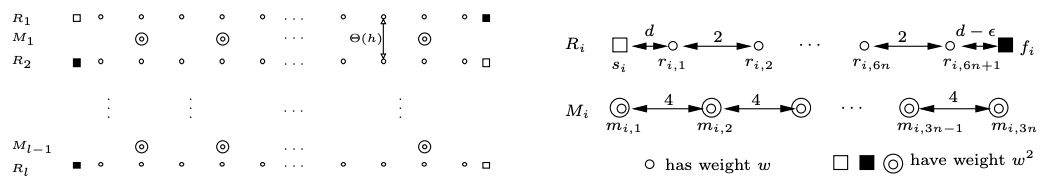
\includegraphics[width=15cm]{chapter_1/files/vattani_fig1.png}
\centering
    \caption{On the left side, the grid of points $H_{l,n}$. On the right, details of the rows \cite{vattani}}
    \label{fig:vattani1}
\end{figure}

\begin{definition}\label{def1}
Define two possible $(3n+2)$-clusterings of $R_i$ ($1\le i \le l$).

$A$: For $1\le j \le 3n$, the $j^{\text{th}}$ cluster of $R_i$ is $\{r_{i,2j-1},r_{i,2j}\}$. It also has the clusters $\{s_i\}$ and $\{r_{i,6n+1},f_i\}$.

$B$: For $1\le j \le 3n$, the $j^{\text{th}}$ cluster of $R_i$ is $\{r_{i,2j},r_{i,2j+1}\}$. It also has the clusters $\{s_i,r_{i,1}\}$ and $\{f_i\}$.
\end{definition}

\begin{definition}\label{def2}
We say that a $k$-clustering of $H_{l,n}$ is ``nice'' if each $m_{i,j}$ is a singleton cluster and each $R_i$ is grouped in an $A$-clustering or in a $B$-clustering.
\end{definition}

\begin{lemma}\label{lem1}
A nice $k$-clustering of $H_{l,n}$ with $t$ rows grouped in an $A$-clustering costs $L_1-t\alpha$.
\end{lemma}

A nice clustering, defined in Definition \ref{def2}, corresponds naturally to the $k$ that was chosen, since there are $l-1$ $M$ rows, each with $3n$ points in singleton clusters, and $l$ $R$ rows, with $3n+2$ clusters each, corresponding to $3n+1$ clusters with two consecutive points and 1 cluster with one point (whether $s_i$ or $f_i$ is the singleton cluster depends on whether $R_i$ is in an $A$ or $B$ clustering, respectively). Note an $A$ clustering saves exactly $\alpha$ cost compared to a $B$ clustering.

\begin{lemma}\label{lem2}
For $w=\text{poly}(n,l)$ large enough, any non-nice $k$-clustering of $H_{l,n}$ costs at least $L_1+\Omega(w)$. On the other hand, any nice $k$-clustering of $H_{l,n}$ costs at most $L_1$.
\end{lemma}

Lemma \ref{lem2} establishes that for $w$ large enough, any optimal clustering of $H_{l,n}$ must be ``nice.'' Note that Lemma \ref{lem1} allows us to make the stronger statement that in additional to the optimal clustering being nice, all $R_i$'s will be grouped in $A$ clusterings, for a total cost of $L_1-l\alpha$.

%However, note that soon we will be adding more points to create $G_{l,n}\cup X$, and for this augmented instance, we will argue that iff the corresponding X3C instance is satisfiable, the optimal clustering will have exactly $n$ $R_i$ in the $A$ clustering and the remaining $R_i$ in the $B$ clustering.

Now we construct the $k$-means instance corresponding to the reduction. It contains the points $G_{l,n}\cup X$, where $G_{l,n}$ is a slightly modified version of $H_{l,n}$ and the set $X=\bigcup_{i=1}^l X_i$ depends on the X3C collection $\mathcal{C}$.

\begin{figure}
    \centering
    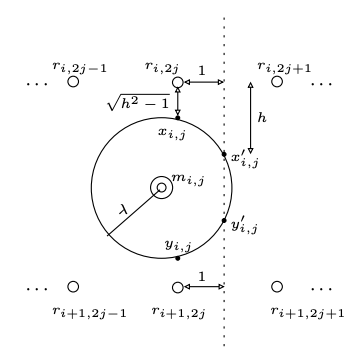
\includegraphics[width=6cm]{chapter_1/files/vattani_fig2.png}
\centering
    \caption{Close-up of $G_{l,n}\cup X$ \cite{vattani}}
    \label{fig:vattani2}
\end{figure}

Refer to Figure \ref{fig:vattani2} for details on $G_{l,n}$, where we set $\lambda=\Theta(h)$ (again, its exact value is only important to the proof of the lemmas which we omit here). The new grid $G_{l,n}$ is identical to $H_{l,n}$ except that the points in the rows in $M_i$ are no longer vertically aligned with the points in the rows $R_i$. The previous results about $H_{l,n}$ still apply to $G_{l,n}$, since the distance between rows is still $\Theta(h)$.

Now we define the set $X$. The spots $x_{i,j},x'_{i,j},y_{i,j},y'_{i,j}$ ($1\le i \le l-1$ and $1 \le j \le 3n$) are not all points in $X$ but rather possible positions of points, where exactly half of each group of four points will be occupied: $x_{i,j}\in X_i\iff j\not\in S_i$; $x'_{i,j}\in X_i\iff j\in S_i$; $y_{i,j}\in X_i\iff j\not\in S_{i+1}$; $y'_{i,j}\in X_i\iff j\in S_{i+1}$. All these points have weight $1$.

We set the number of clusters to be the same $k$ as before, and the cost limit to $L=L_1+L_2-n\alpha$ where $L_2=6n(l-1)h^2\frac{2w}{2w+1}$.

\begin{definition}\label{def3}
A cluster $C$ is ``good'' for a point $z\not\in C$ if adding $z$ to $C$ increases the cost by exactly $h^2\frac{2w}{2w+1}$.
\end{definition}

\begin{lemma}\label{lem3}
For any $1\le j \le 3n$, $1\le i \le l-1$, the following holds:
\begin{itemize}
    \item The clusters $\{m_{i,j}\}$, $\{r_{i,2j-1},r_{i,2j}\}$, and $\{r_{i,2j},r_{i,2j+1}\}$ are good for $x_{i,j}$.
    \item The clusters $\{m_{i,j}\}$, $\{r_{i+1,2j-1},r_{i+1,2j}\}$, and $\{r_{i+1,2j},r_{i+1,2j+1}\}$ are good for $y_{i,j}$.
    \item The clusters $\{m_{i,j}\}$ and $\{r_{i,2j},r_{i,2j+1}\}$ are good for $x'_{i,j}$.
    \item The clusters $\{m_{i,j}\}$ and $\{r_{i+1,2j},r_{i+1,2j+1}\}$ are good for $y'_{i,j}$.
\end{itemize}
\end{lemma}

Note that we have added $\abs{X}=6n(l-1)$ additional points and that if $j\in S_i$, then the corresponding $x'_{i,j}$ and $y'_{i-1,j}$ will only have a ``good'' cluster in $R_i$ if $R_i$ has a $B$ clustering, whereas $j\not\in S_i$ does not impose this restriction on the corresponding $x_{i,j}$ and $y_{i-1,j}$, i.e. $R_i$ can have either an $A$ or $B$ clustering.

Definition \ref{def3} and Lemma \ref{lem3} justify the choice of $L_2$. Also, from Figure \ref{fig:vattani2}, we can verify that the ``good'' clusters mentioned in Lemma \ref{lem3} are indeed the closest clusters to the spots $x_{i,j},x'_{i,j},y_{i,j},y'_{i,j}$.

\begin{lemma}\label{lem4}
Consider any optimal $k$-clustering of $G_{l,n}\cup X$. Then for $w=\text{poly}(n,l)$ large enough, the clustering induced on $G_{l,n}$ is nice and the points in $X$ are in different good clusters.
\end{lemma}

See \cite{vattani} for proofs of Lemmas \ref{lem1}, \ref{lem2}, \ref{lem3}, and \ref{lem4}. The following final lemma contains the reduction.

\begin{lemma}\label{lem5}
The set $G_{l,n}\cup X$ has a $k$-clustering of cost less or equal to $L$ if and only if there is an exact cover $\mathcal{F}\subseteq \mathcal{C}$ for the X3C instance.
\end{lemma}

\begin{proof}
$(\implies)$ Suppose we have an optimal $k$-clustering with cost $\le L$. Define $\mathcal{F}=\{S_i:R_i\text{ is grouped in an $A$ clustering}\}$. We argue that $\mathcal{F}$ is an exact cover of $U$. Note that $|\mathcal{F}|\ge n$ since $L = L_1+L_2-n\alpha$. It is sufficient to prove that the sets in $\mathcal{F}$ do not overlap, since this means that $|\mathcal{F}| = n$ and furthermore $\bigcup_{S\in\mathcal{F}}S=U$. 

Consider some $S_i\in\mathcal{F}$ and some $j\in S_i$. Since we know that $R_i$ has an $A$-clustering, the $j^{\text{th}}$ cluster of $R_i$ is not a good cluster for any point in $X$. Then we make a pigeonhole-like argument: each $j$ ($1\le j \le 3n$) corresponds to $2(l-1)$ points in $X$. For these points, there are $l-1$ ``good'' clusters in $M$ rows and $l$ ``good'' clusters in $R$ rows (corresponding to the $j^{\text{th}}$ cluster in $R_i$ for $1\le i\le l$). So if the $j^{\text{th}}$ cluster in $R_i$ is not occupied by any point, then the $j^{\text{th}}$ cluster in all $R_{i'}$, $i'\ne i$, must be occupied by some point. For a given $i'\ne i$, the only candidates are the points in $X$ with the subscript $_{i',j}$, and therefore it must be that either $R_{i'}$ has a $B$-clustering (allowing for both $x/y$ or $x'/y'$ type points) or $j\not\in S_{i'}$, and then we know that the points will be the less restrictive $x/y$ type. This proves that $j\not\in S_{i'}$ for any $S_{i'}\in\mathcal{F}$ where $i'\ne i$, i.e. the sets in $\mathcal{F}$ do not overlap.

$(\impliedby)$ Suppose X3C has an exact cover $\mathcal{F}$. We define a $k$-clustering for $G_{l,n}\cup X$. Place all points $m_{i,j}$ into different singleton clusters. For each $1\le i \le l$, make $R_i$ an $A$-clustering if $S_i\in\mathcal{F}$ and a $B$-clustering otherwise. For each $1\le j \le 3n$, let $i(j)$ be the (unique) index such that $j\in S_{i(j)}$ and $S_{i(j)}\in\mathcal{F}$. For each $i<i(j)$, merge $x_{i,j}$ (or $x'_{i,j}$) with the $j^{\text{th}}$ cluster of $R_i$ and merge $y_{i,j}$ (or $y'_{i,j}$) with $\{m_{i,j}\}$. For each $i\ge i(j)$, merge $x_{i,j}$ (or $x'_{i,j}$) with $\{m_{i,j}\}$ and merge $y_{i,j}$ (or $y'_{i,j}$) with the $j^{\text{th}}$ cluster of $R_{i+1}$.

We will show that this assignment has cost at most $L$, which means that the answer to our $k$-means decision problem is yes. This happens if we have a ``nice'' clustering on the points in $G_{l,n}$, there are $n$ $R_i$ rows in $A$ clusterings, and all points in $X$ are assigned to different good clusters. The first two are explicitly satisfied in the construction; we only need to verify that in cases where we assigned $x'_{i,j}$ (resp. $y'_{i,j}$) where $1\le i < i(j)$ (resp. $i\ge i(j)$), it was indeed to a good cluster. However, if $x'_{i,j}$ (resp. $y'_{i,j}$) $\in X_i$, then $j\in S_i$ (resp. $S_{i+1}$), and since the sets in $\mathcal{F}$ are nonoverlapping, this means $S_i$ (resp. $S_{i+1}$) $\not\in\mathcal{F}$, and therefore $R_i$ (resp. $R_{i+1}$) is a $B$ clustering. Therefore all points were assigned to good clusters.
\end{proof}
